\begin{figure}[htbp]
\centering
% 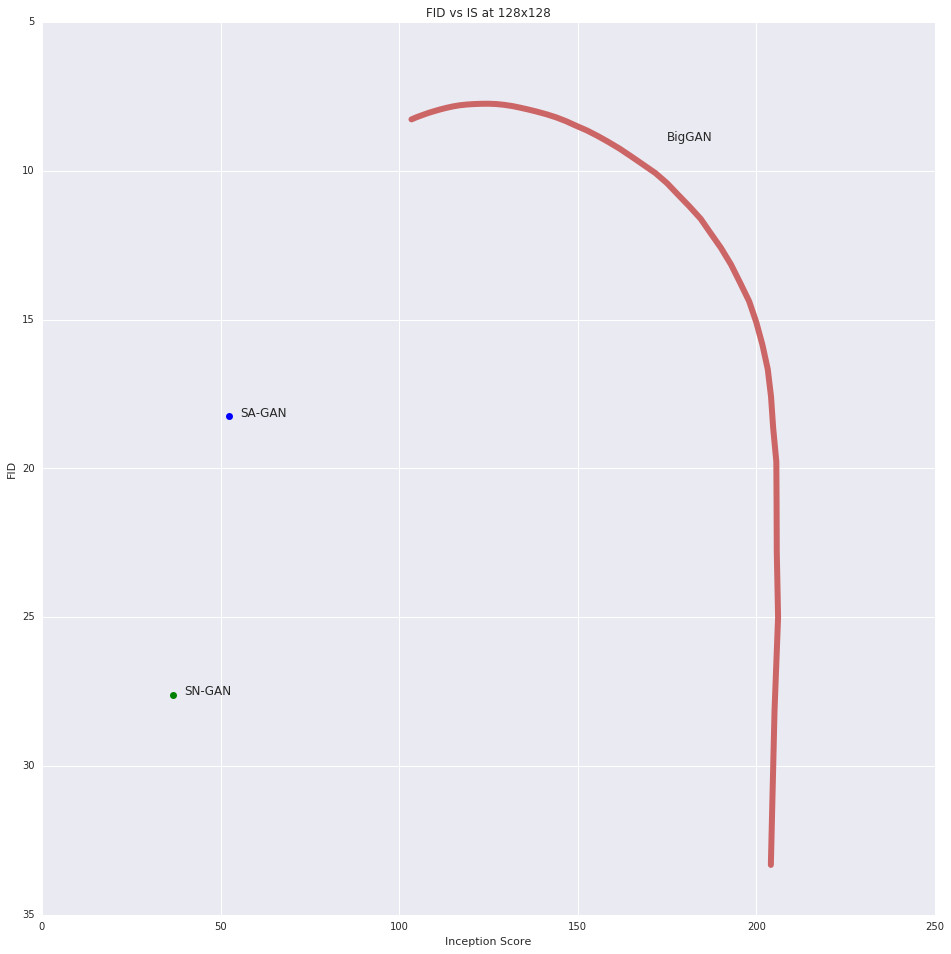
\includegraphics[width=0.85\textwidth]{images/ISvFID128a.png}
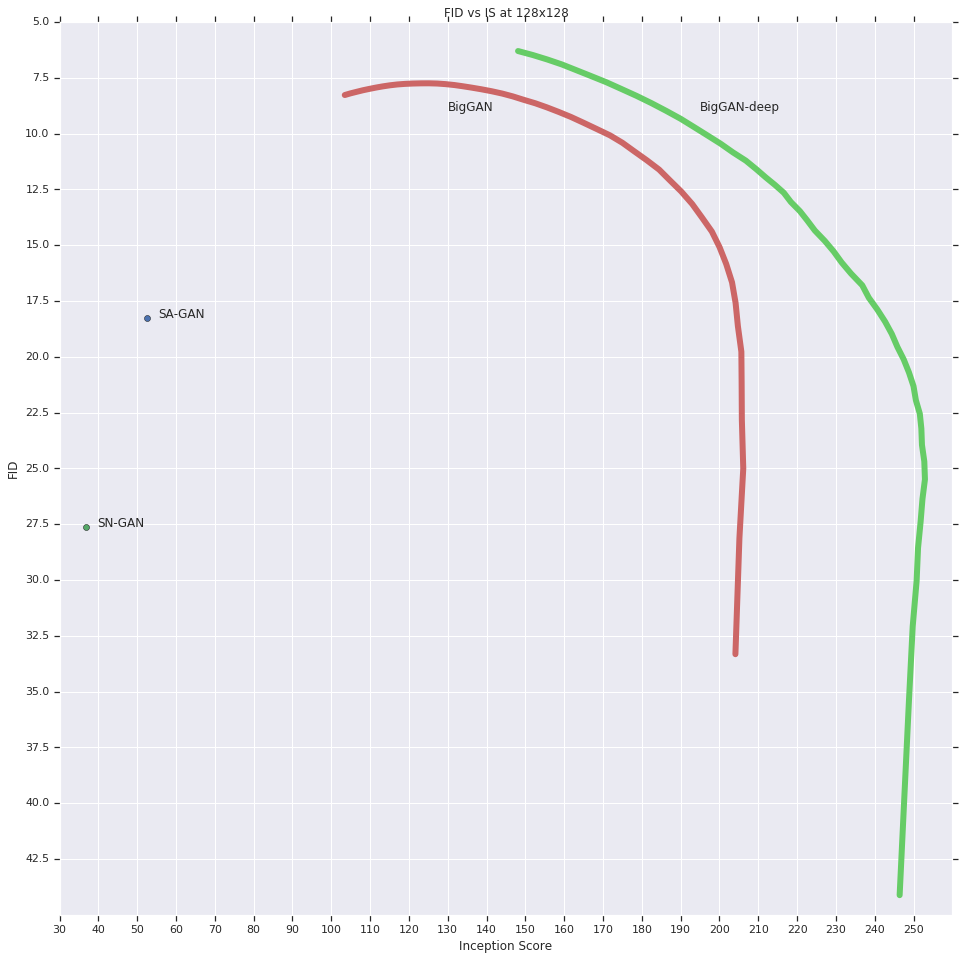
\includegraphics[width=0.85\textwidth]{images/BigGAN-deep_ISvFID_128.png} 
\caption{IS vs. FID at 128$\times$128. Scores are averaged across three random seeds.}
\label{appendix_ISvFID128}
\end{figure}


\begin{figure}[htbp]
\centering
\begin{tabular}{cc}
% 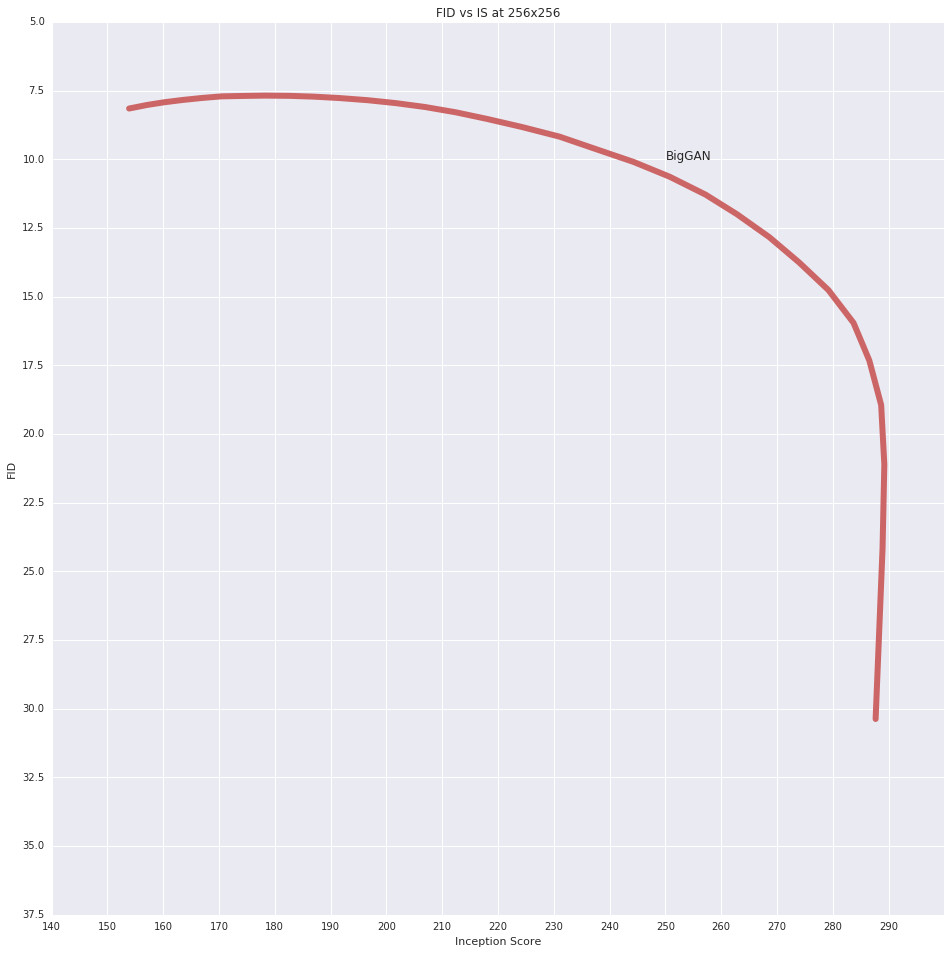
\includegraphics[width=0.47\textwidth]{images/ISvFID256b.png} &
% 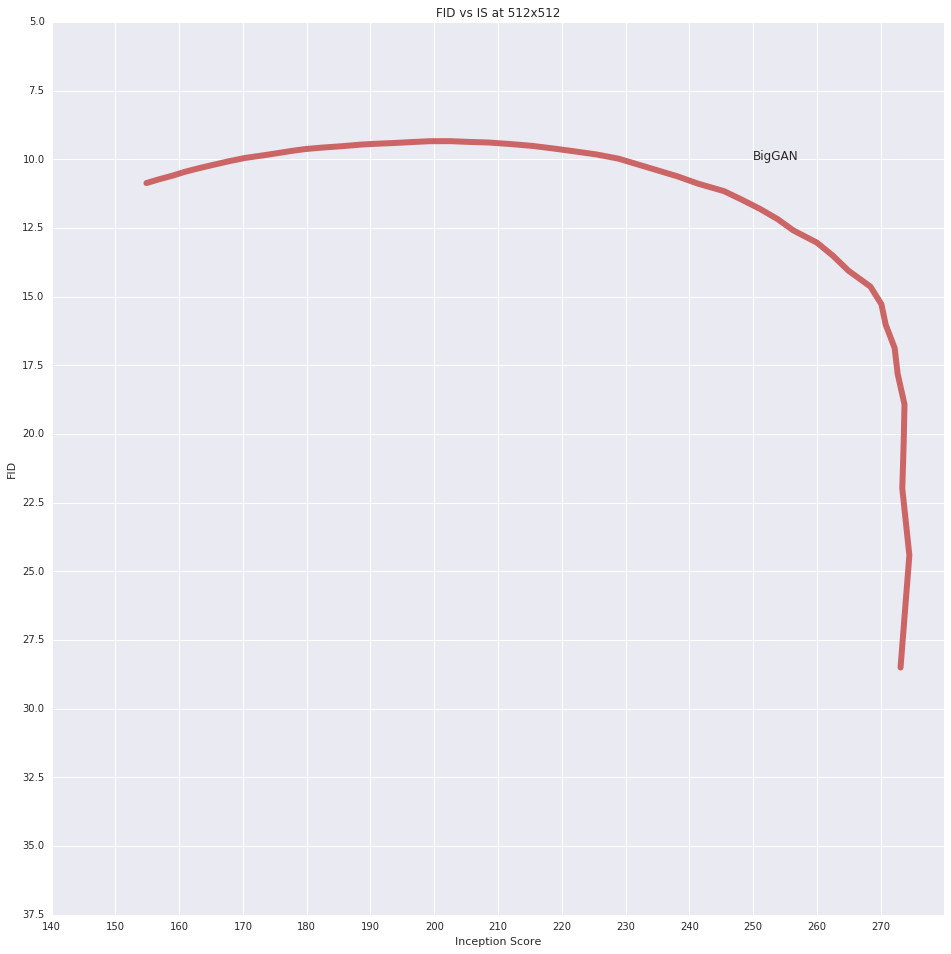
\includegraphics[width=0.47\textwidth]{images/ISvFID512a.png}
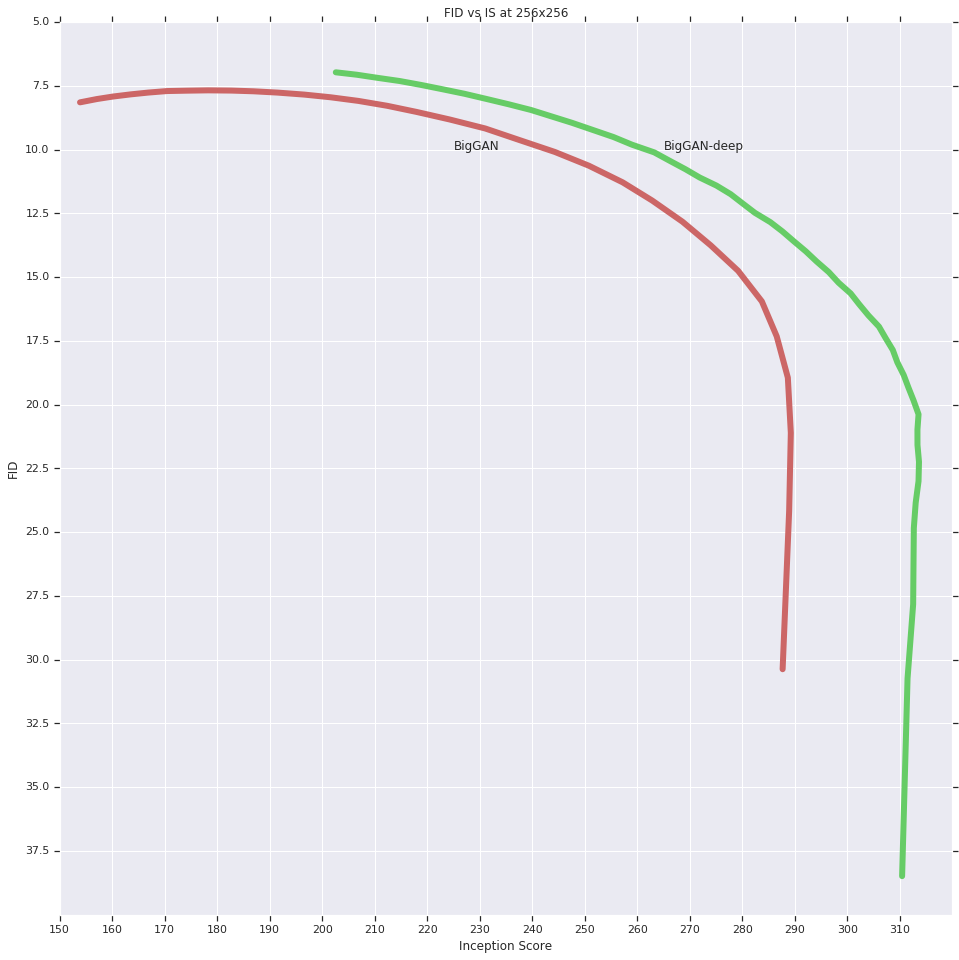
\includegraphics[width=0.47\textwidth]{images/BigGAN-deep_ISvFID_256.png} &
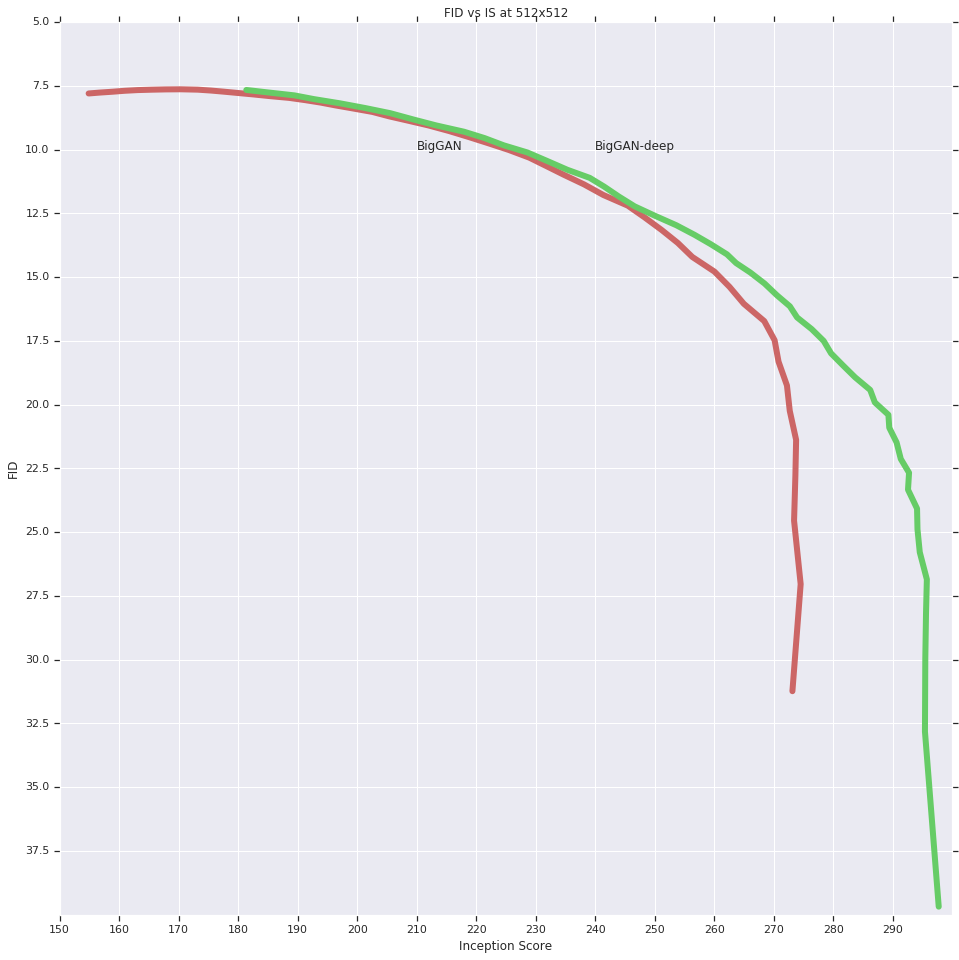
\includegraphics[width=0.47\textwidth]{images/BigGAN-deep_ISvFID_512.png} 
\end{tabular}
\caption{IS vs. FID at 256 and 512 pixels. Scores are averaged across three random seeds for 256.}%$\times$256.}
\label{appendix_ISvFID256}
\end{figure}

\begin{figure}[htbp]
\centering
\begin{tabular}{c}
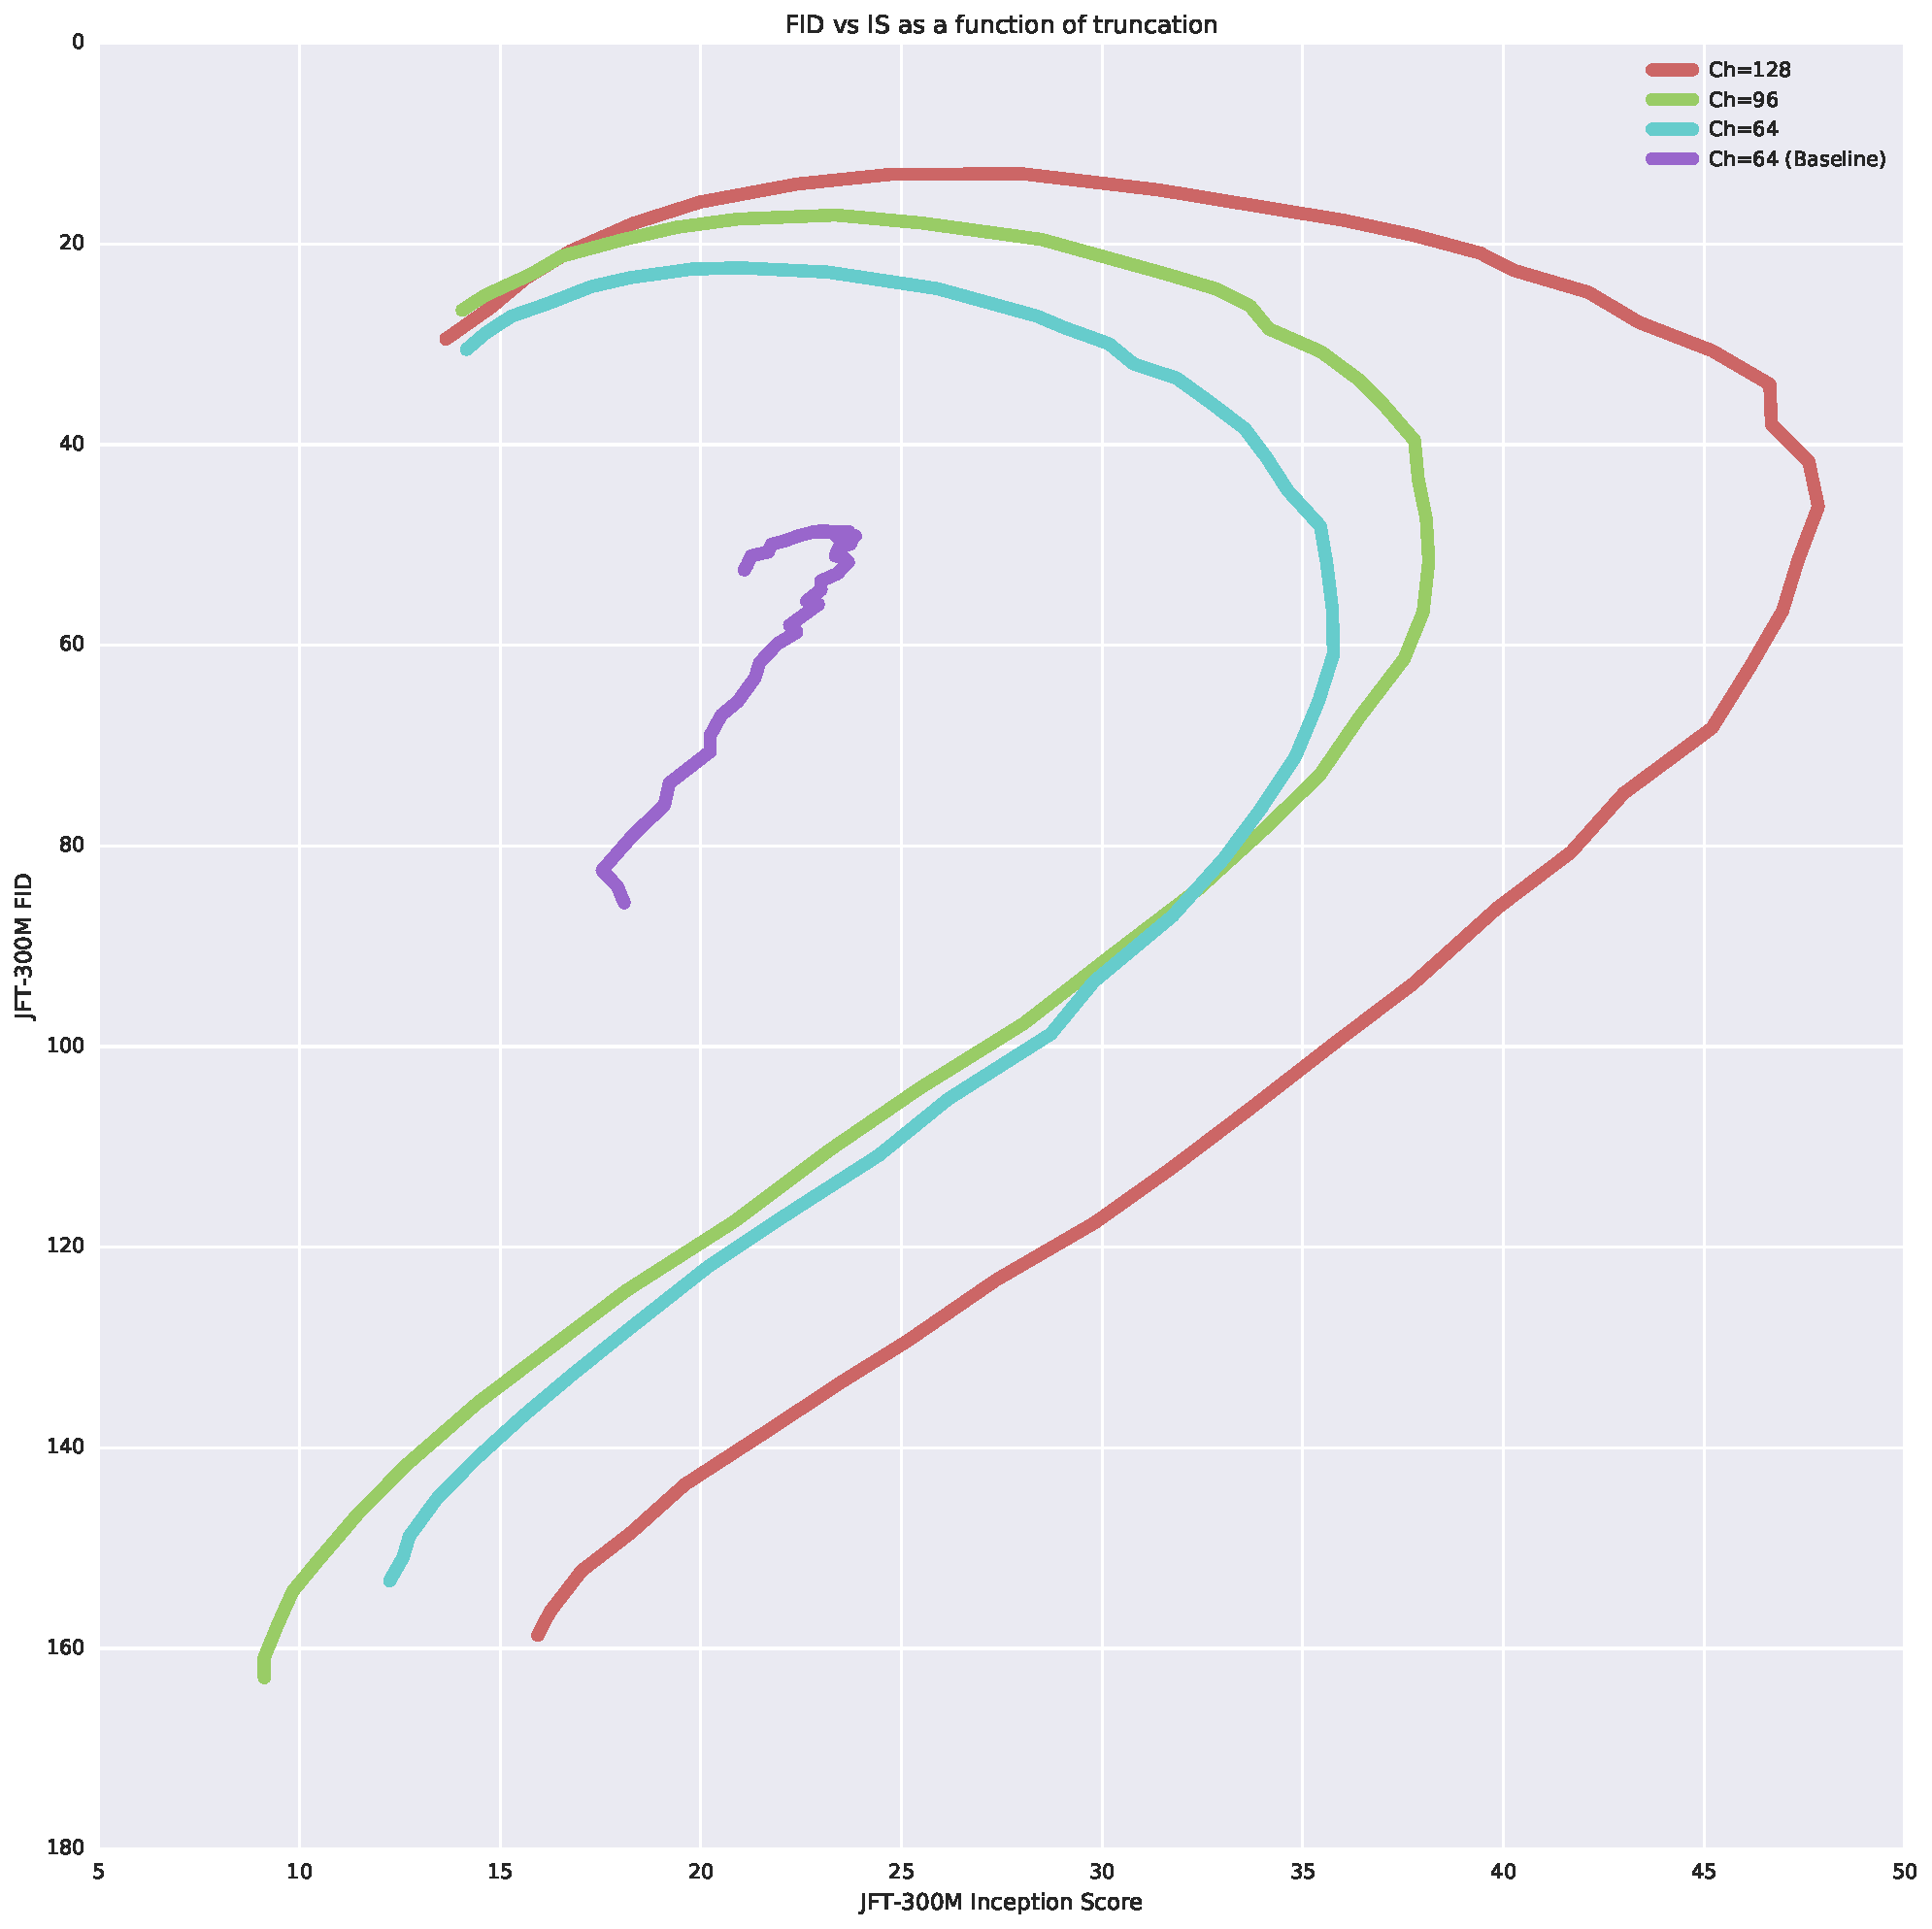
\includegraphics[width=0.65\textwidth]{images/jft_truncation_curves/jft_truncation_curve_256.pdf} \\
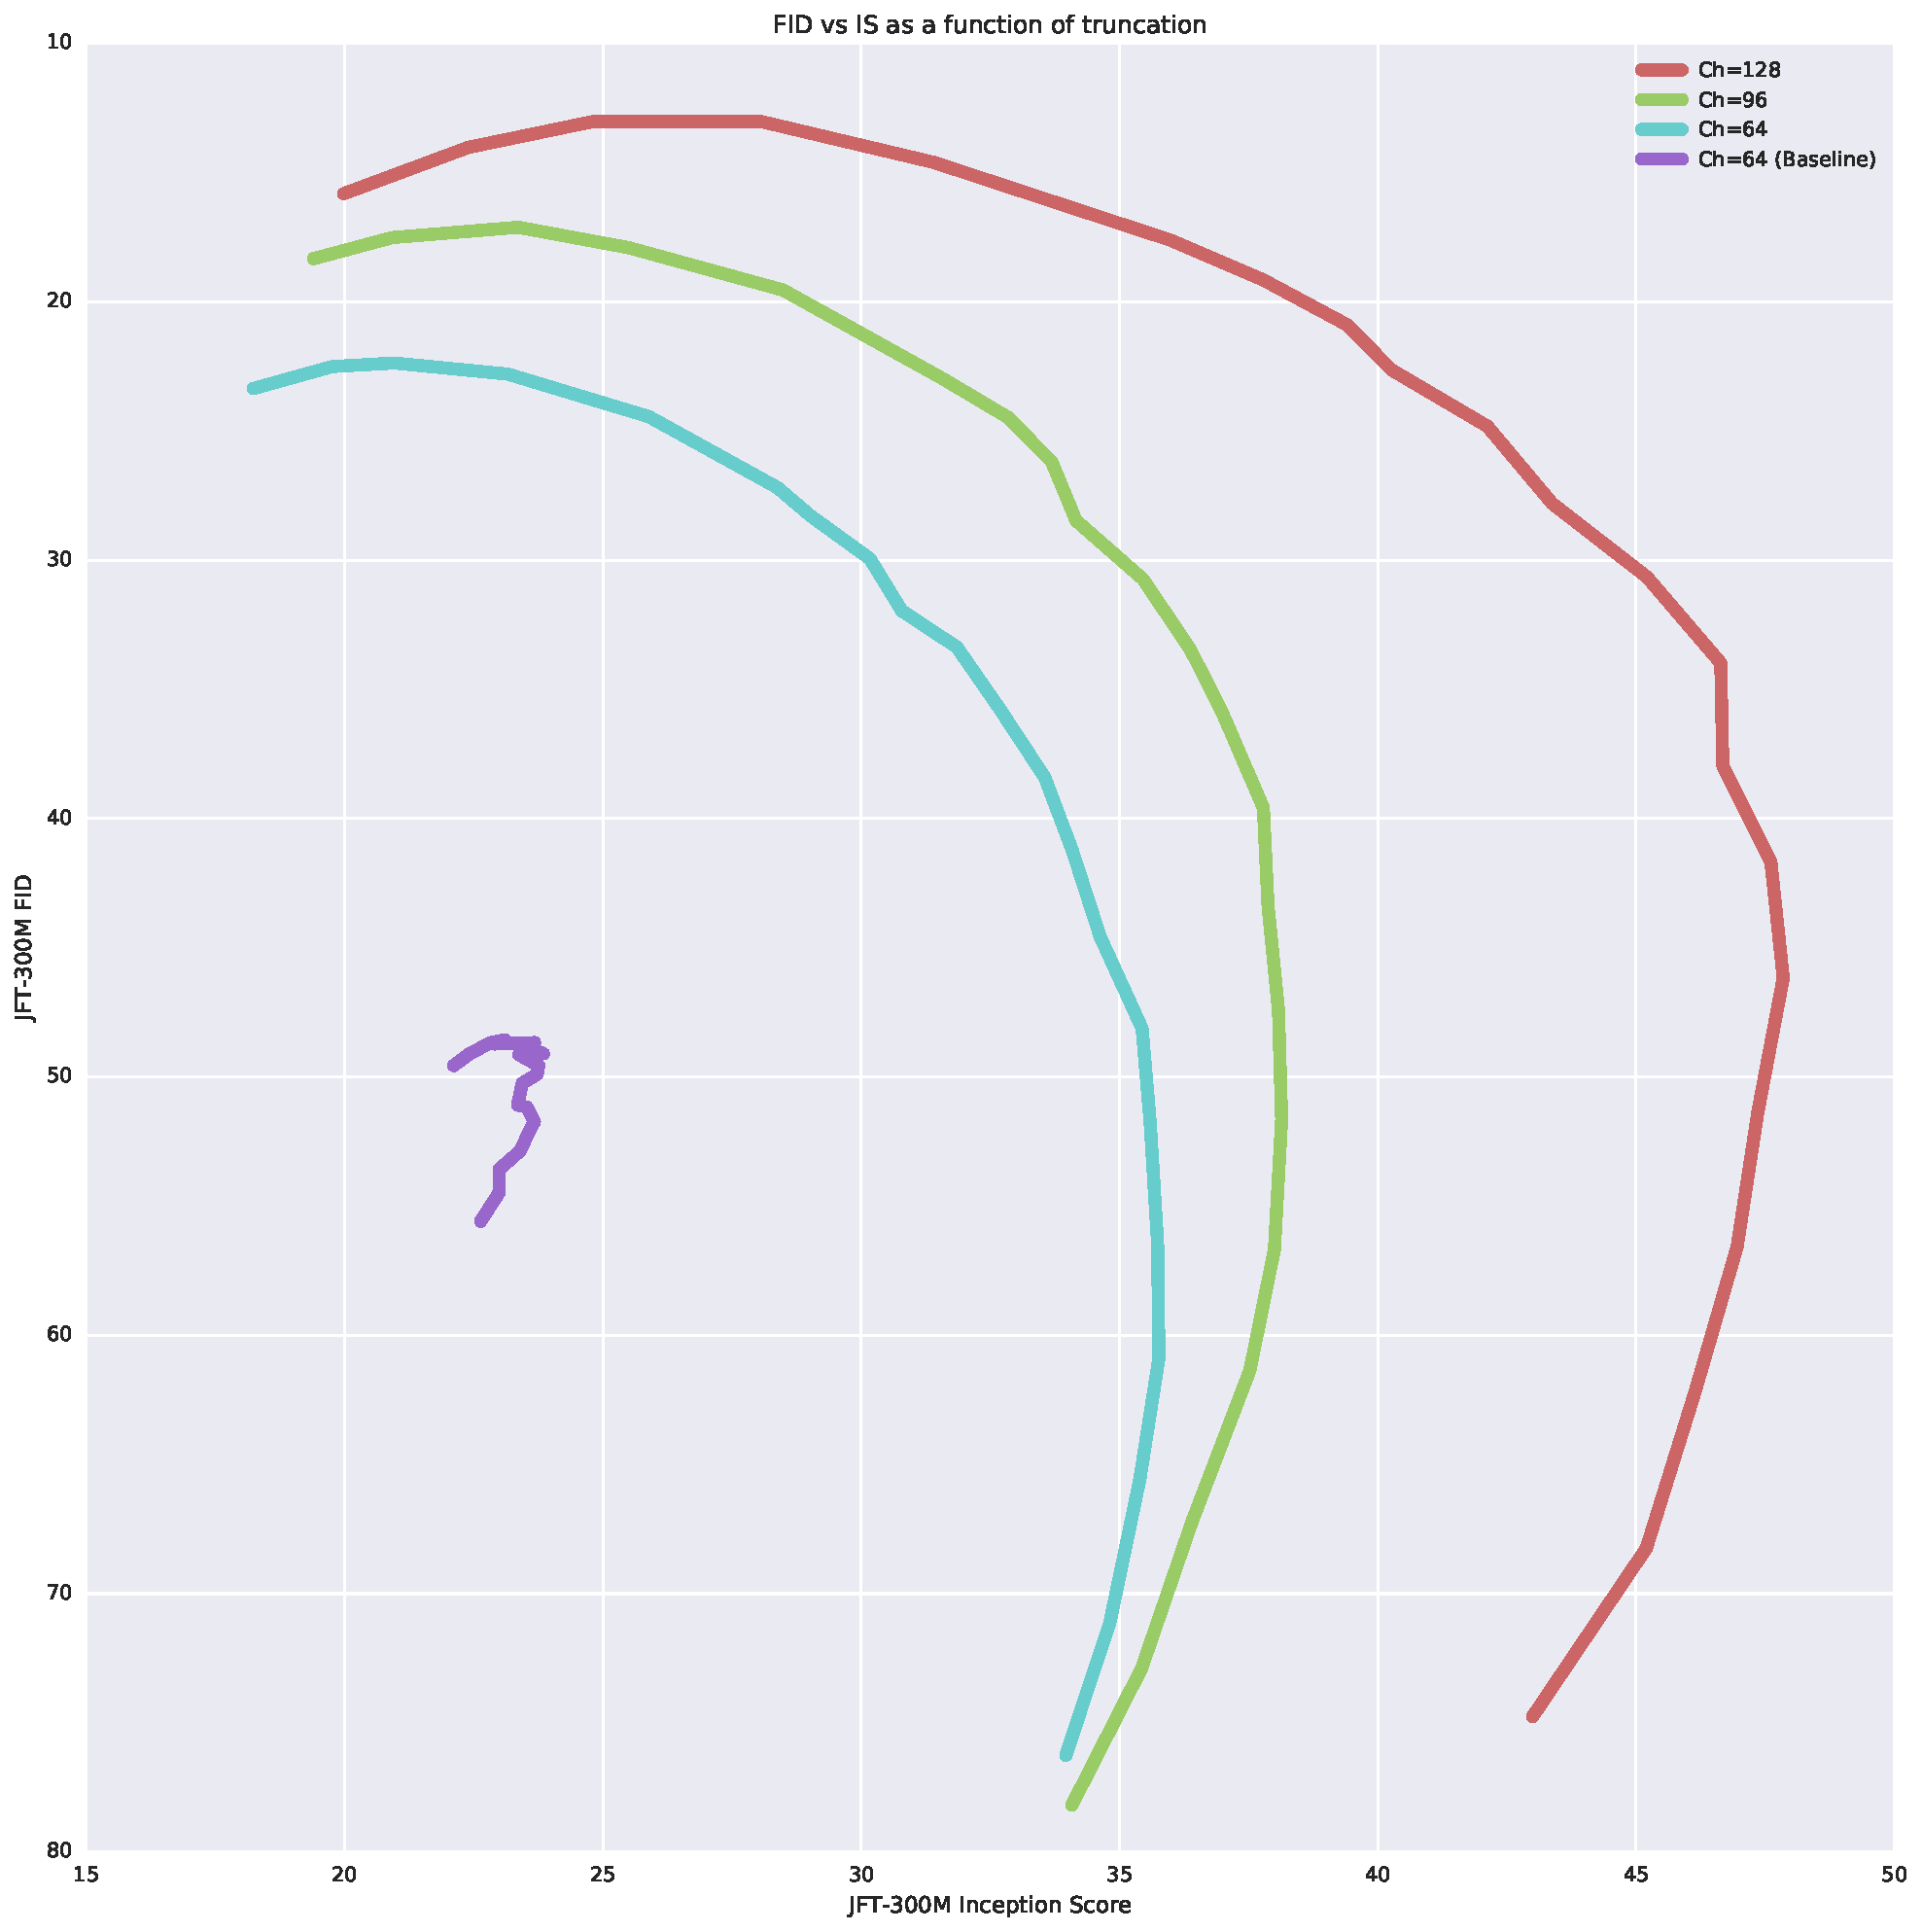
\includegraphics[width=0.65\textwidth]{images/jft_truncation_curves/jft_truncation_curve_256_0p5_1p5.pdf}
%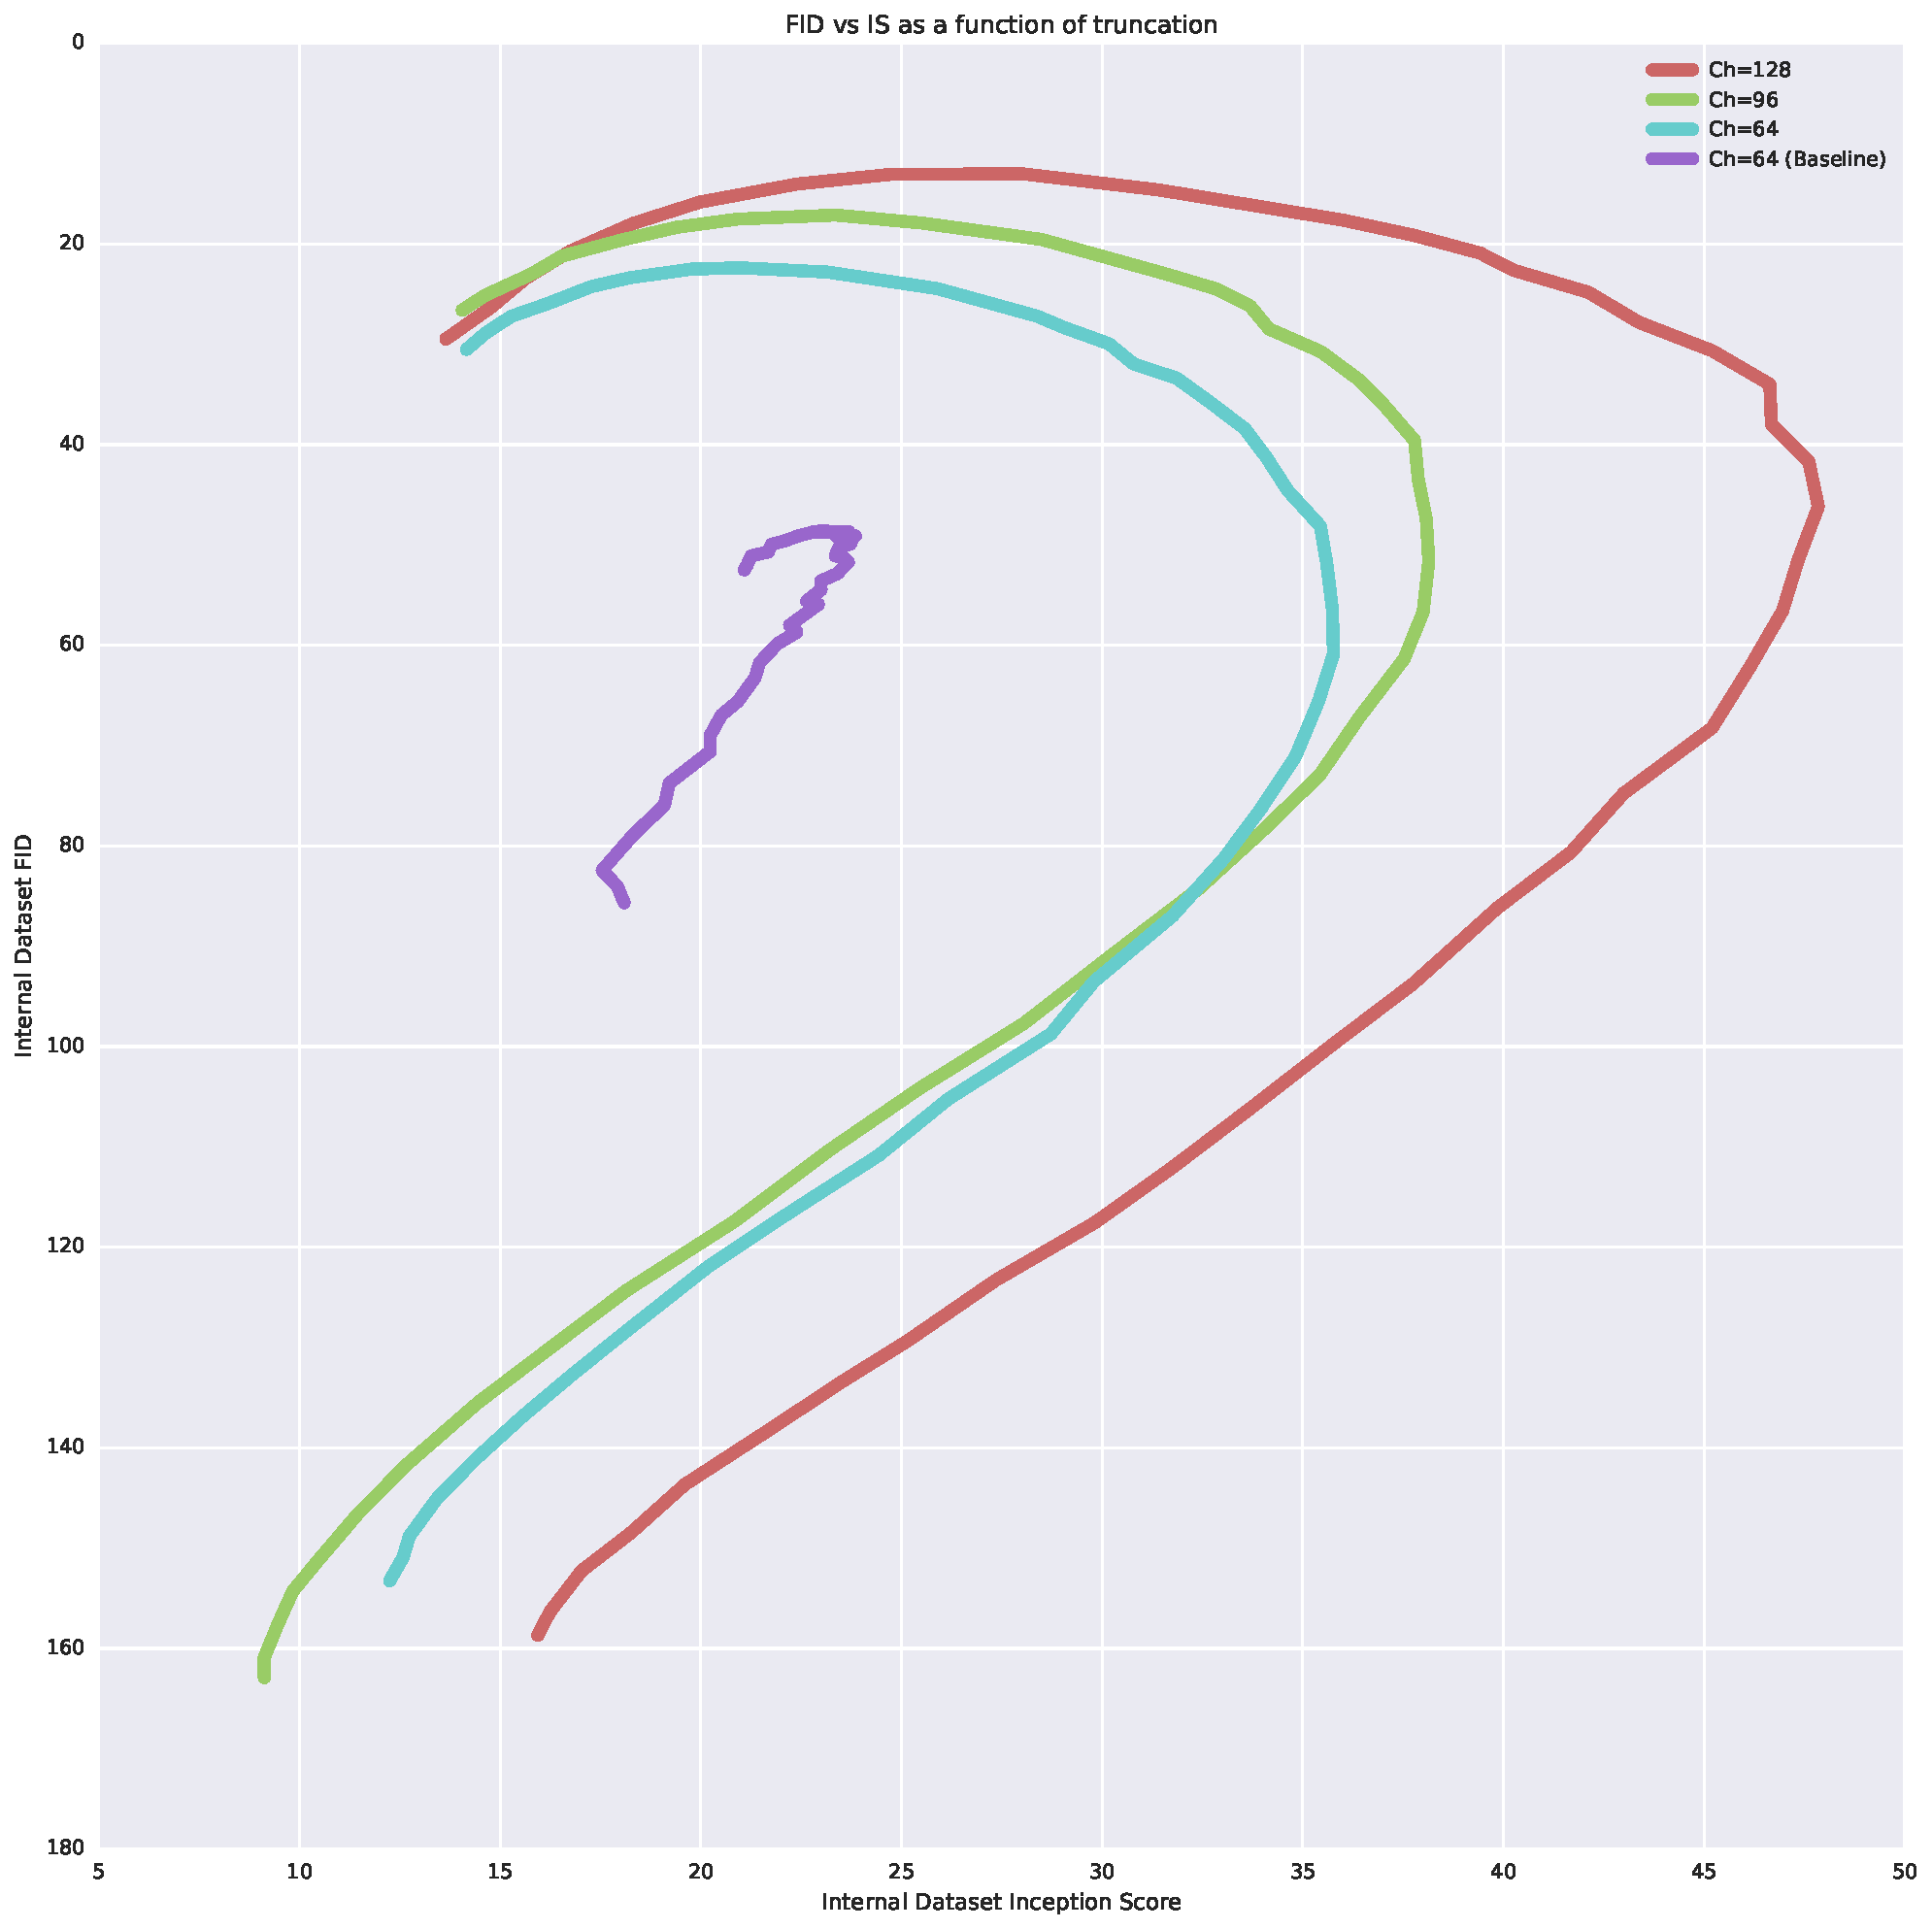
\includegraphics[width=0.65\textwidth]{images/jft_truncation_curves/anon_jft_truncation_curve_256.pdf} \\
%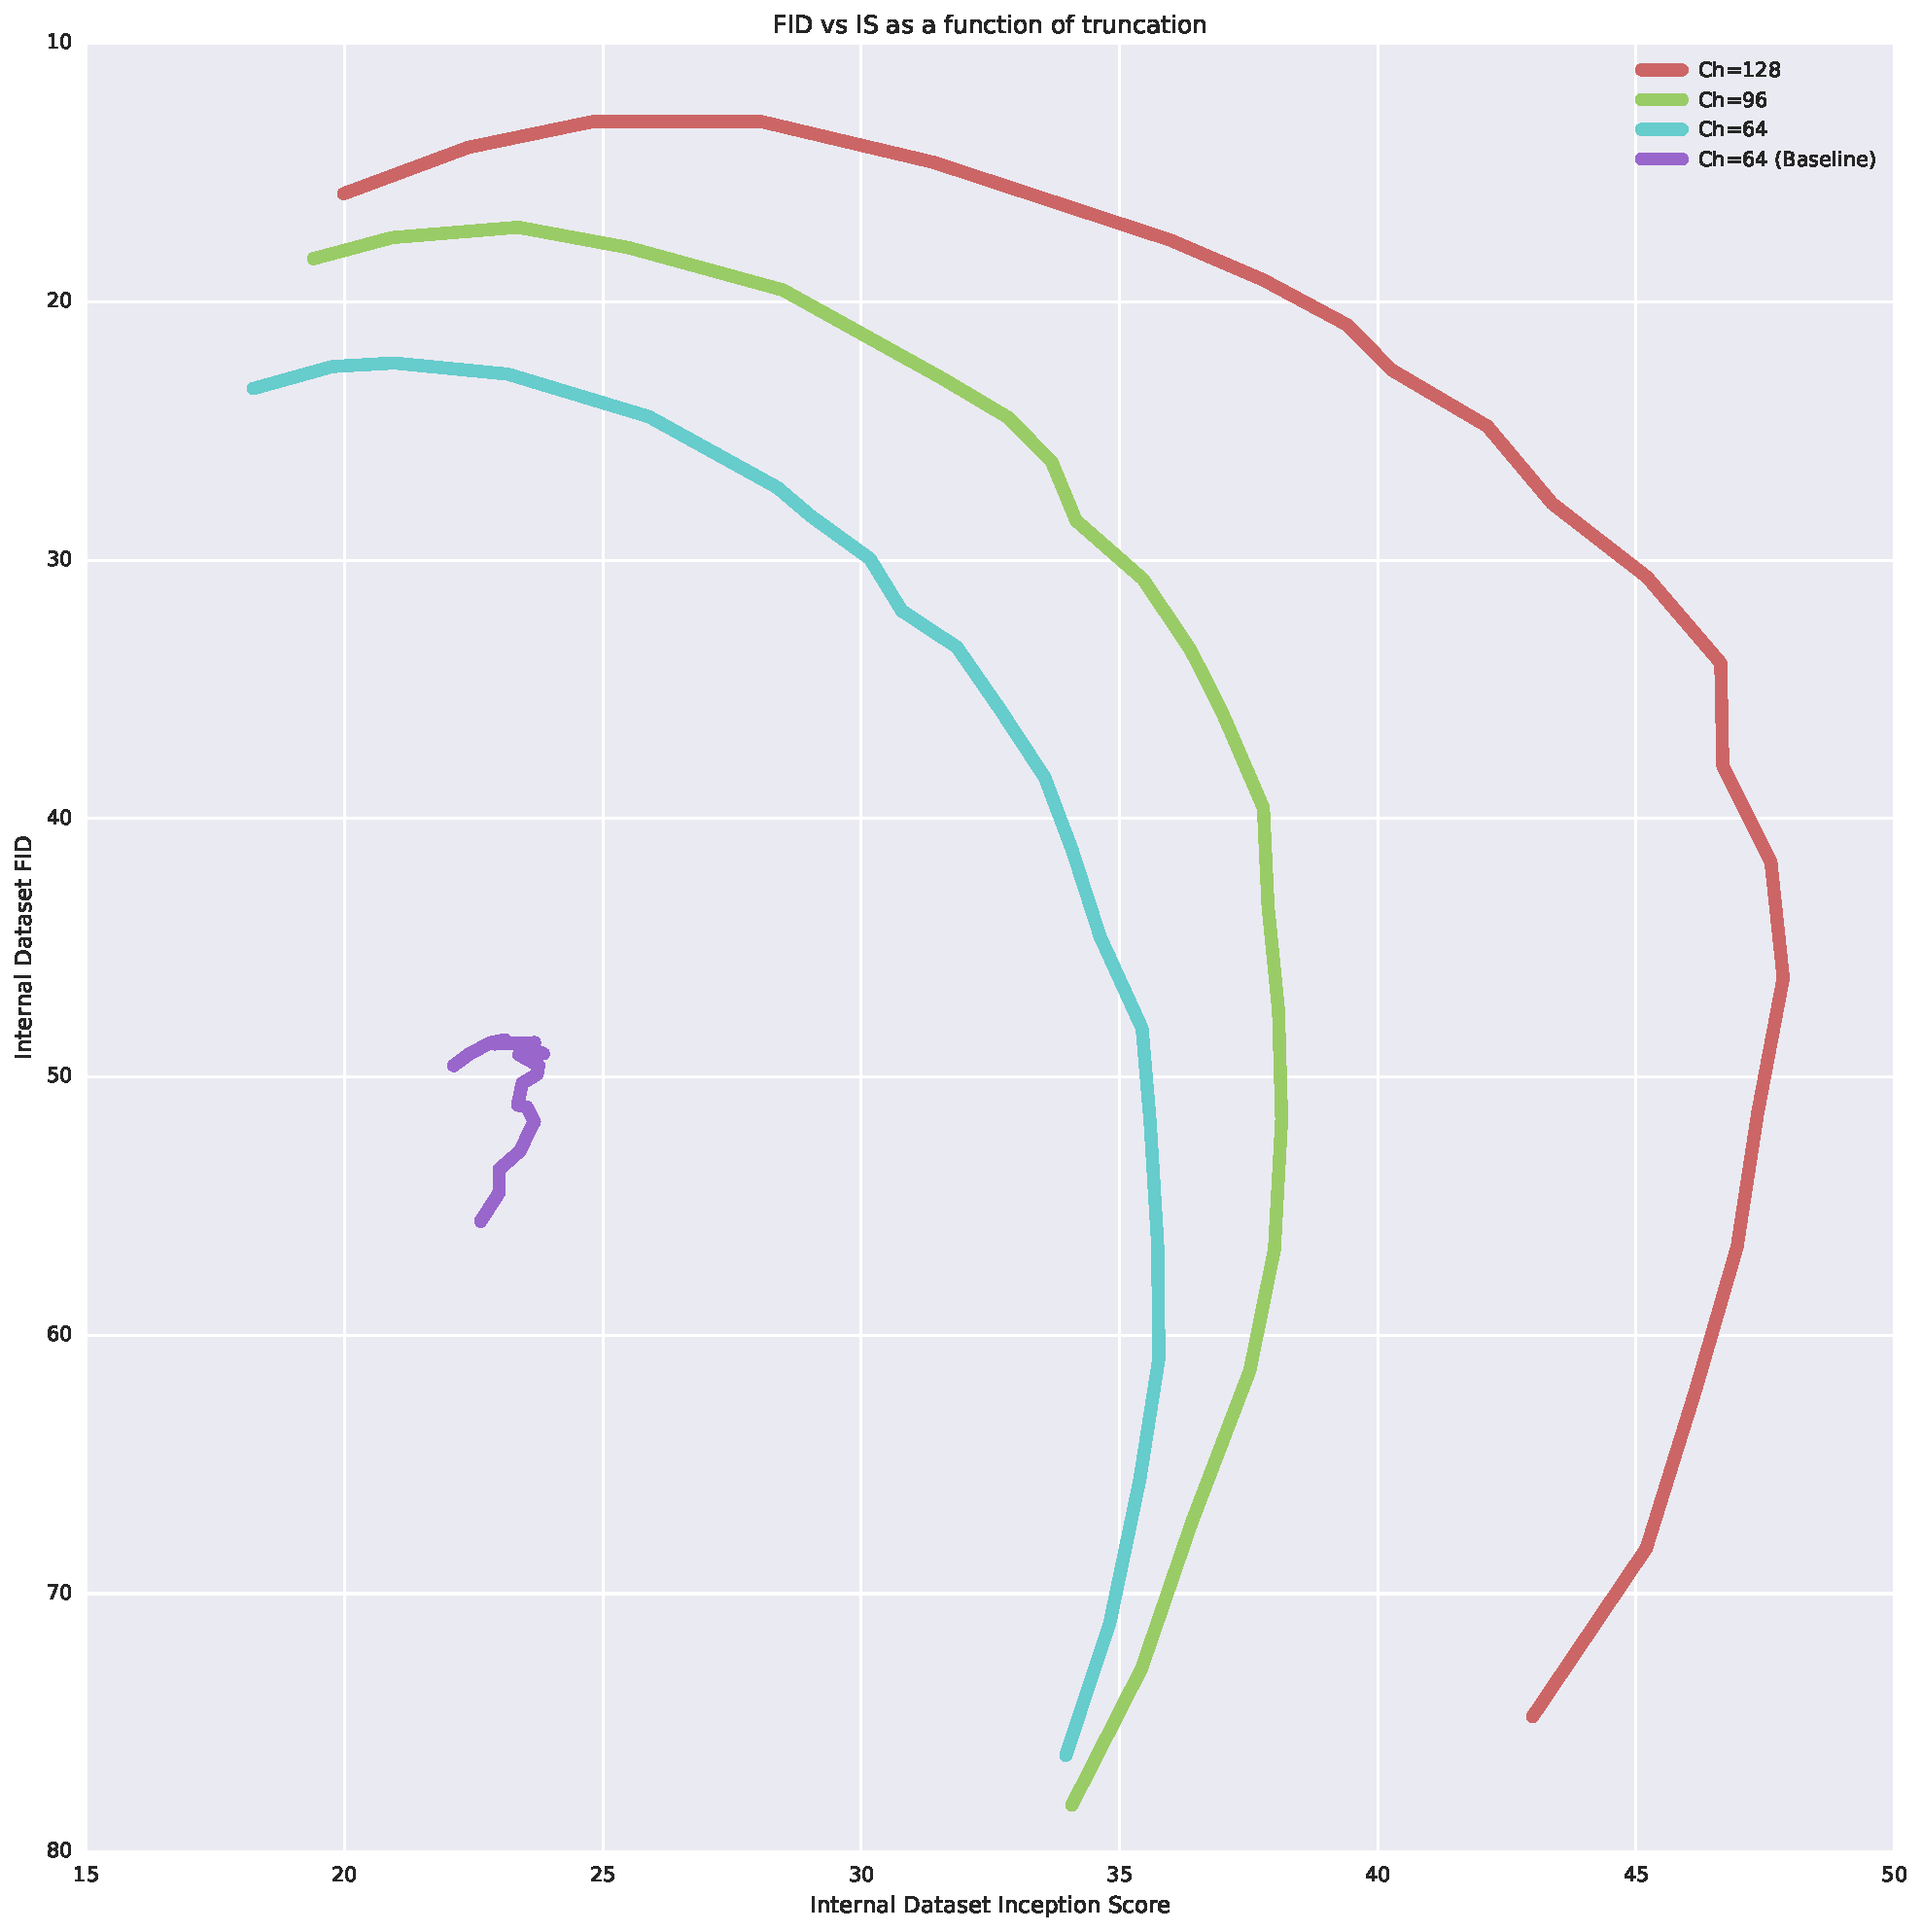
\includegraphics[width=0.65\textwidth]{images/jft_truncation_curves/anon_jft_truncation_curve_256_0p5_1p5.pdf}
\end{tabular}
\caption{
JFT-300M IS vs. FID at 256$\times$256.
%IS vs. FID for the internal dataset at 256$\times$256.
We show truncation values from $\sigma = 0$ to $\sigma = 2$ (top) 
and from $\sigma = 0.5$ to $\sigma = 1.5$ (bottom).
Each curve corresponds to a row in Table~\ref{jft_table}.
The curve labeled with \textit{baseline} corresponds to the first row (with orthogonal regularization and other techniques disabled), while the rest correspond to rows 2-4 -- the same architecture at different capacities (\textit{Ch}). 
\label{appendix_jft_trunc}
}
\end{figure}